\documentclass[12pt]{article}
\usepackage[spanish,es-tabla]{babel}
\usepackage{natbib}
\usepackage{url}
\usepackage{float}
\usepackage[utf8]{inputenc}
\usepackage{amsmath}
\usepackage{graphicx}
\usepackage{fancyhdr}
\usepackage{longtable}
\usepackage{vmargin}
\usepackage{listings}
\usepackage{hyperref}
\usepackage{multirow}
\usepackage{xcolor}
\usepackage{caption}
\usepackage{subcaption}

\colorlet{punct}{red!60!black}
\definecolor{background}{HTML}{EEEEEE}
\definecolor{delim}{RGB}{20,105,176}
\colorlet{numb}{magenta!60!black}

\lstdefinelanguage{json}{
    basicstyle=\normalfont\ttfamily,
    numbers=left,
    numberstyle=\scriptsize,
    stepnumber=1,
    numbersep=8pt,
    showstringspaces=false,
    breaklines=true,
    frame=lines,
    backgroundcolor=\color{background},
    literate=
      *{:}{{{\color{punct}{:}}}}{1}
      {,}{{{\color{punct}{,}}}}{1}
      {\{}{{{\color{delim}{\{}}}}{1}
      {\}}{{{\color{delim}{\}}}}}{1}
      {[}{{{\color{delim}{[}}}}{1}
      {]}{{{\color{delim}{]}}}}{1},
}

\setmarginsrb{3 cm}{2.5 cm}{3 cm}{2.5 cm}{1 cm}{1.5 cm}{1 cm}{1.5 cm}

\title{Tarea - 04}
\date{\today}

\makeatletter
\let\thetitle\@title
\let\theauthor\@author
\let\thedate\@date
\makeatother

\pagestyle{fancy}
\fancyhf{}
\rhead{\theauthor}
\lhead{\thetitle}
\cfoot{\thepage}

\addto\captionsspanish{
  \renewcommand{\contentsname}%
    {Tabla de contenido}%
}

\begin{document}
    \pagestyle{fancy}
    \fancyhf{}

    \lhead{\begin{picture}(0,0) \put(0,0){
\includegraphics[width=30mm]{images/Logo2.png}} \end{picture}}
    \renewcommand{\headrulewidth}{0.7pt}
    \fancyhead[R]{Detección de temas en tendencia}
\fancyfoot[R]{\thepage}

\begin{titlepage}
	\centering
    
\includegraphics[scale = 0.45]{images/Logo.png}\\[0.5 cm]	% University Logo
    \textsc{\large Universidad de los Andes\\
        \vspace{0.2cm} 
        Facultad de Ingeniería\\
        \vspace{0.3cm} 
        Proyecto final}\\[2.0 cm]	% University Name
	\textsc{\Large Procesamiento de lenguaje natural}\\[0.5 cm]
	% Course Code
	\rule{\linewidth}{0.2 mm} \\[0.4 cm]
	{ \LARGE \bfseries \thetitle}\\
	\rule{\linewidth}{0.2 mm} \\[1.5 cm]
	
	\large
			\emph{Presentado por:} \\
			Juan David García Hernández\\
			Nicolás Rocha Pacheco\\
			César Daniel Garrido Urbano\\
			
	\vfill
	\large
			\emph{Presentado a:}\\
			Rubén Francisco Manrique Pirmanrique\\
\end{titlepage}

\thispagestyle{empty}
\tableofcontents
\pagebreak

\setcounter{page}{1}
\section{Introducción}
La clasificación de texto es un área de investigación del procesamiento de lenguaje natural que se define como el problema de identificar y asignar una serie de categorías predefinidas a un conjunto de archivos. Según \cite{mokey_learn}, tiene un amplio campo de aplicaciones como análisis de sentimientos, etiquetado de temas, detección de \textit{spam}, detección de postura, entre otros.\\

La famosa red social \textit{Twitter} implementa algoritmos de clasificación de temas en sus \textit{tweets} con el fin e resaltar los temas más discutidos momento a momento. No obstante, una de las funciones más útiles de estos algoritmos es para etiqueta de datos. Actualmente, la inteligencia artificial y el procesamiento de lenguaje natural funcionan especialmente bien cuando se pueden entrenar los modelos sobre datos etiquetados. No obstante, la etiqueta de dichos datos es un proceso laborioso y tedioso en especial cuando se tiene una gran cantidad de datos (lo cual es ideal para mejorar el desempeño del modelo).\\

Se han propuesto numerosas técnicas y algoritmos que buscan clasificar texto, en especial enfocándose una correcta extracción de características, haciendo uso de diferentes métodos y modelos del estado del arte. A continuación, se presenta una revisión bibliográfica, la metodología y procedimiento a implementar en este proyecto y finalmente resultados y conclusiones sobre el \textit{set} de datos utilizados.

\newpage
\newpage

\section{Revisión bibliográfica}
Tratando explícitamente el tema de detección de temas en \textit{Twitter} los autores de  \cite{ReviewApproachesTopcicDetection} realizan un recuento de diferentes métodos que buscan solucionar el problema. Inicia por explicar y comparar acercamientos tradicionales que varían en la manera en que se representan los temas que son tendencia: la estrategia pivot de documentos los representa como un agrupamiento de documentos mientras que pivot de características los representa como un agrupamiento de palabras claves.\\

Posteriormente presenta una tabla que resume la manera en que diferentes algoritmos propuestos dan solución resaltando características del mismo: \textit{embedding} o no \textit{embedding}, eventos específicos o no específicos, y detección supervisada y no supervisada. Profundizando en la primera comparación, la diferencia radica en qué tipo de modelos se utilizan para la representación de las palabras. Los métodos que no utilizan \textit{embeddings} implementan modelos como \textit{Bag of Words} o \textit{TF-IDF}, los cuales según \cite{ReviewApproachesTopcicDetection} sufren de poca capacidad de generalización, dado, entre otros, a que se basa en la re-ocurrencia de palabras, lo cual en documentos cortos resulta poco probable. Por su parte la utilización de \textit{embeddings} consiste en la representación continua de palabras en un idioma mapeándolas como vectores de un espacio dimensional bajo. Esta técnica es más reciente y ofrece mejores resultados en varias tareas de procesamiento de lenguaje natural. Siguiendo con las diferencias, los eventos indican la información que se conoce de cada observación del conjunto de datos, como por ejemplo localización, hora, fecha, etc. La tercera categoría depende de si la detección es supervisada o no supervisada, dependiendo de si se poseen las etiquetas correctas de cada observación o no. Esto incide ampliamente en el tipo de modelo de \textit{Machine Learning} a utilizar.\\

En \cite{TrendTopicsDetectionFromTwitter} y \cite{FuzzyIncrementalTopicDetection} se presentan diferentes aproximaciones de agrupamiento de temas y tendencias haciendo extracción de palabras claves de cada documento. Inician por el preprocesamiento en donde se remueven caracteres especiales y puntuación, lematización. Posteriormente se descubren vectores de temas aplicando HDA (Hierarchical Dirichlet Processes) y se utiliza para encontrar la distribución de tópicos en cada tweets, donde el que tiene mayor probabilidad corresponde al tema tendencia. Finalmente, para cada uno de los grupos de temas se crea un grafo de dependencia entre \textit{tweets} midiendo la similaridad de los mismos.\\

En \cite{DeepRepresentationClusteringTweets} y \cite{UnsupervisedDeepEmbeddingClustering} muestran las ventajas y beneficio en los resultados que se puede obtener a través de la utilización de modelos profundos, como autoencoders y redes neuronales del estado del arte como Bert, para obtener un \textit{embedding} más adecuado y que finalmente beneficia el método de agrupamiento utilizado. Estas últimas referencias muestran algo de la tendencia actual en la gran mayoría de retos del procesamiento de lenguaje natural, pues antes de proponer nuevos algoritmos de clasificación o \textit{clustering} se ha procurado desarrollar y mejorar las herramientas que se utilizan para representar matemáticamente los documentos.

\section{Metodología y procedimiento}

En la figura \ref{fig:TopicDetectionDiag} se presenta la metodología propuesta para resolver la tarea de detección de tópicos a través de una representación de palabras con modelos profundos y técnicas de \textit{clustering}. Esta metodología se inspiro principalmente en el trabajo presentados en \cite{DeepRepresentationClusteringTweets}, en donde no solo se utiliza el modelo BERT para hacer la representación de las palabras sino que esto combina con un \textit{autoencoder} para reducir la dimensionalidad de las representaciones. No obstante, dadas las limitaciones de computación y de tiempo, no se utilizaron las representaciones de todas las palabras, ni un autoencoder basado en redes convolucionales 2D, sino que se implementó una aproximación más sencilla del mismo modelo, la cual se explica más adelante en esta sección. Asimismo, para poder hacer una descripción de los tópicos (resultado de las agrupaciones hechas por el algoritmo de \textit{clustering}), se tomaron ideas de \cite{TrendTopicsDetectionFromTwitter}, al buscar las palabras claves de cada \textit{cluster} y representarlas en una nube de palabras. Finalmente, se hizo un análisis de estos resultados a nivel de las agrupaciones obtenidas y el comportamiento a lo largo del tiempo, lo cual permitió ajustar los parámetros de cada una de las distintas etapas de procesamiento y obtener resultados presentados.

\begin{figure}[H]
    \centering
    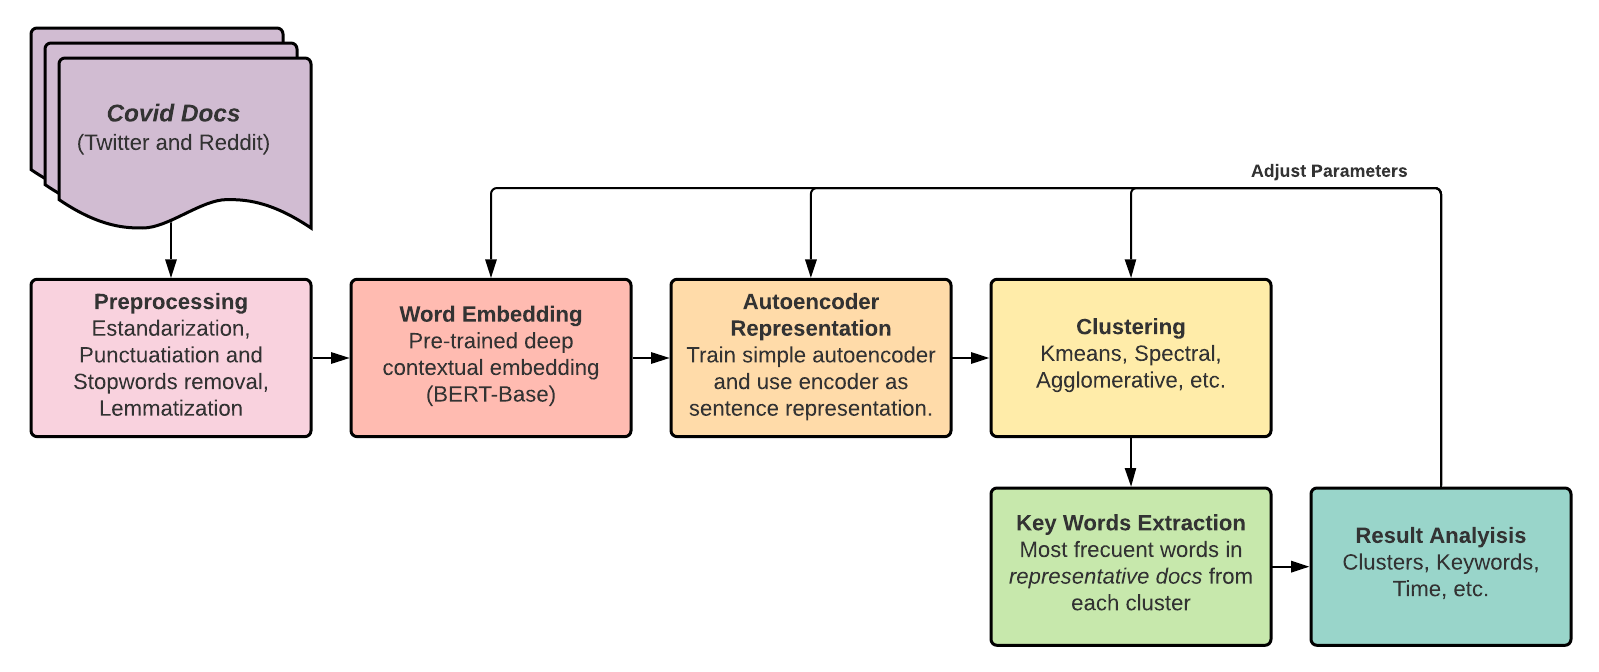
\includegraphics[width=\textwidth]{doc_hw04/images/TopicDetectionDiag.png}
    \caption{Metodología propuesta para la detección de tópicos utilizando \textit{deep sentence representation} y \textit{clustering}.}
    \label{fig:TopicDetectionDiag}
\end{figure}

\subsection{Dataset}
El \textit{dataset} utilizado para detección de temas en tendencia corresponde documentos recogidos por los autores de dos fuentes diferentes \textit{Twitter} y \textit{Reddit} en inglés, español y francés. Por cuestión de tiempo de procesamiento se decidió excluir las noticias recopiladas. Si bien se tiene una gran cantidad de datos en inglés (más de 800.00 documentos) se decide utilizar únicamente alrededor de 135.000 datos con el fin de impedir que la cantidad de documentos favoreciera un idioma por encima de otro, y poder analizar con mayor imparcialidad. El total de documentos utilizados en cada caso se muestra en la tabla \ref{tab:docs}.

\begin{table}[H]
\centering
\caption{Total de documentos utilizados por idioma}
\label{tab:docs}
\begin{tabular}{lrrrr}
\hline
\textbf{Idioma} & \textbf{Twitter} & \textbf{Reddit} & \textbf{Total} \\ \hline
Inglés          & 99.971           & 45.725          & 145.696        \\
Español         & 125.000          & 6.479           & 131.479        \\
Francés         &                  &                 &                \\ \hline
\end{tabular}
\end{table}

\subsection{Preprocesamiento}

El preprocesamiento de los datos se realizó siguiendo los siguientes pasos:
\begin{enumerate}
    \item Pasar todas las palabras a minúsculas.
    \item Eliminar signos de puntuación y caracteres especiales.
    \item Tokenizar las palabras.
    \item Lematizar las palabras.
\end{enumerate}

\begin{itemize}
    \item \textbf{Reddit original:}
    \begin{itemize}
        \item [\textbf{Inglés:}] Someone I am close to works in a factory called Dixon in Maryland. This person is one of only 2 people wearing a mask in the entire factory, including office staff. How this is acceptable I have no idea. The recklessness and denial in the face of a global pandemic is astounding. Companies not protecting employees in close proximity with masks wearing policy should be fined. It's criminal given what we know about transmission.
        \item [\textbf{Español:}] INER está al 100\% de capacidad por COVID y personal está agotado, advierte su director.
        \item [\textbf{Francés:}] Pourquoi autant mentir? On veut freiner et éliminer la contagion au Québec ou la nourrir comme on arrose un jardin? Je comprends pas.
    \end{itemize}
    \item \textbf{Reddit preprocesado:}
    \begin{itemize}
        \item [\textbf{Inglés:}] 'someone', 'close', 'works', 'factory', 'called', 'dixon', 'maryland', 'person', 'one', '2', 'people', 'wearing', 'mask', 'entire', 'factory', 'including', 'office', 'staff', 'acceptable', 'idea', 'recklessness', 'denial', 'face', 'global', 'pandemic', 'astounding', 'companies', 'protecting', 'employees', 'close', 'proximity', 'masks', 'wearing', 'policy', 'fined', 'criminal', 'given', 'know', 'transmission'
        \item [\textbf{Español:}]'iner', '100', 'capacidad', 'covid', 'personal', 'agotado', 'advierte', 'director'.
        \item [\textbf{Francés:}] 'pourquoi', 'autant', 'mentir', 'veut', 'freiner', 'éliminer', 'contagion', 'québec', 'nourrir', 'comme', 'arrose', 'jardin', 'comprends'
    \end{itemize}
    \item \textbf{Tweet original:}
    \begin{itemize}
        \item [\textbf{Inglés}] \#WorldBank “Living paper”: \#SocialProtection and Jobs - Responses to \#COVID19: A Real-Time Review of Country Measures; version 15 (May 14, 2021)
        \item [\textbf{Español:}] Madrid ha gastado ya, dicen aquí, 299 millones de euros en hacer frente a la pandemia... habiendo recibido 3.384 millones...
        \item [\textbf{Francés:}] La progression de la protection vaccinale contre la covid 19 permettra-t-elle prochainement d'assouplir les recommandations ? \#COVID19 \#VaccinationCovid 
    \end{itemize}
    \item \textbf{Tweet preprocesado:}\\ 
    \begin{itemize}
        \item [\textbf{Inglés:}] 'worldbank', 'living', 'paper', 'socialprotection', 'jobs', 'responses', 'covid19', 'realtime', 'review', 'country', 'measures', 'version', '15', 'may', '14', '2021'
        \item [\textbf{Español:}] 'madrid', 'gastado', 'dicen', 'aquí', '299', 'millones', 'euros', 'hacer', 'frente', 'pandemia', 'recibido', '3384', 'millones'
        \item [\textbf{Francés:}] 'progression', 'protection', 'vaccinale', 'contre', 'covid', '19', 'permettratelle', 'prochainement', 'dassouplir', 'recommandations', 'covid19', 'vaccinationcovid'
    \end{itemize}
\end{itemize}

\subsection{Extracción de características}

Una vez preprocesados los datos se procedió a extraer las características (\textit{o features}) de cada una de las sentencias utilizando un modelo profundo pre-entrenado. Para este trabajo se utilizaron en total 3 versiones de BERT-base pre-entrenadas, una para cada idioma: El modelo 
bertweet-covid19-base-uncased \cite{bertweet} (reentrenado sobre un corpus de 850M de tweets relacionados con las tematicas de covid-19), el modelo de BETO o Spanish BERT \cite{CaneteCFP2020} (reentrenado para idioma español) y finalmente el modelo bert-base-french-europeana-cased (reentrenado para idioma framces). Adicionalmente, se hicieron pruebas sobre el modelo covid-twitter-bert-v2 \cite{muller2020covid}, no obstante, al estar este basado en el BERT-Large, el tiempo de computo era considerablemente mayor por lo que fue necesario descartar dicha opción. \\

Ahora bien, de estos modelos es posible obtener varias representaciones a nivel de palabras o de sentencias con base en los distintos tokens que utiliza el modelo (véase figura \ref{fig:BERT_Tokens}). En este caso, se decidió utilizar como representación de la sentencia el token \texttt{CLS}. Este es un token especial utilizado en la tarea de clasificación y que codifica la información de toda la expresión, en este caso todo el documento (tweet,  post o comentario de Reddit). De esta manera, para cada documento se tendrá un vector asociado a su representación de 768 posiciones. 

\begin{figure}[H]
    \centering
    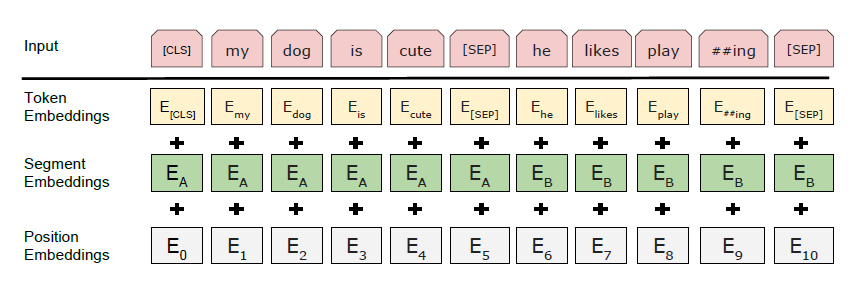
\includegraphics[width=0.8\textwidth]{doc_hw04/images/BERT_Tokens.png}
    \caption{\textit{Tokens} utilizados en el modelo BERT}
    \label{fig:BERT_Tokens}
\end{figure}

No obstante, los algoritmos de \textit{clustering} suelen presentar un mejor funcionamiento en espacios de dimensiones reducidas, esto mejora la convergencia pues da una mejor idea del concepto de distancia. Así las cosas y similar a como se presenta en \cite{DeepRepresentationClusteringTweets} se utiliza un autoencoder para reducir la dimensionalidad de las representaciones (véase figura \ref{fig:autoencoder}). El modelo utilizado no es más que una red neuronal que se entrena con los mismos datos a la entrada y a la salida, lo que internamente comprime y descomprime la información. Esto permite obtener una representación, en un espacio latente mucho menor al de la entrada (en este caso se paso de 768 a 32 dimensiones), que contiene suficiente información para reconstruir la misma información en la salida. Así las cosas, es esta información codificada la que se utilizó como entrada al modelo de agrupación o \textit{clustering} para realizar la detección no supervisada de tópicos.

\begin{figure}[H]
    \centering
    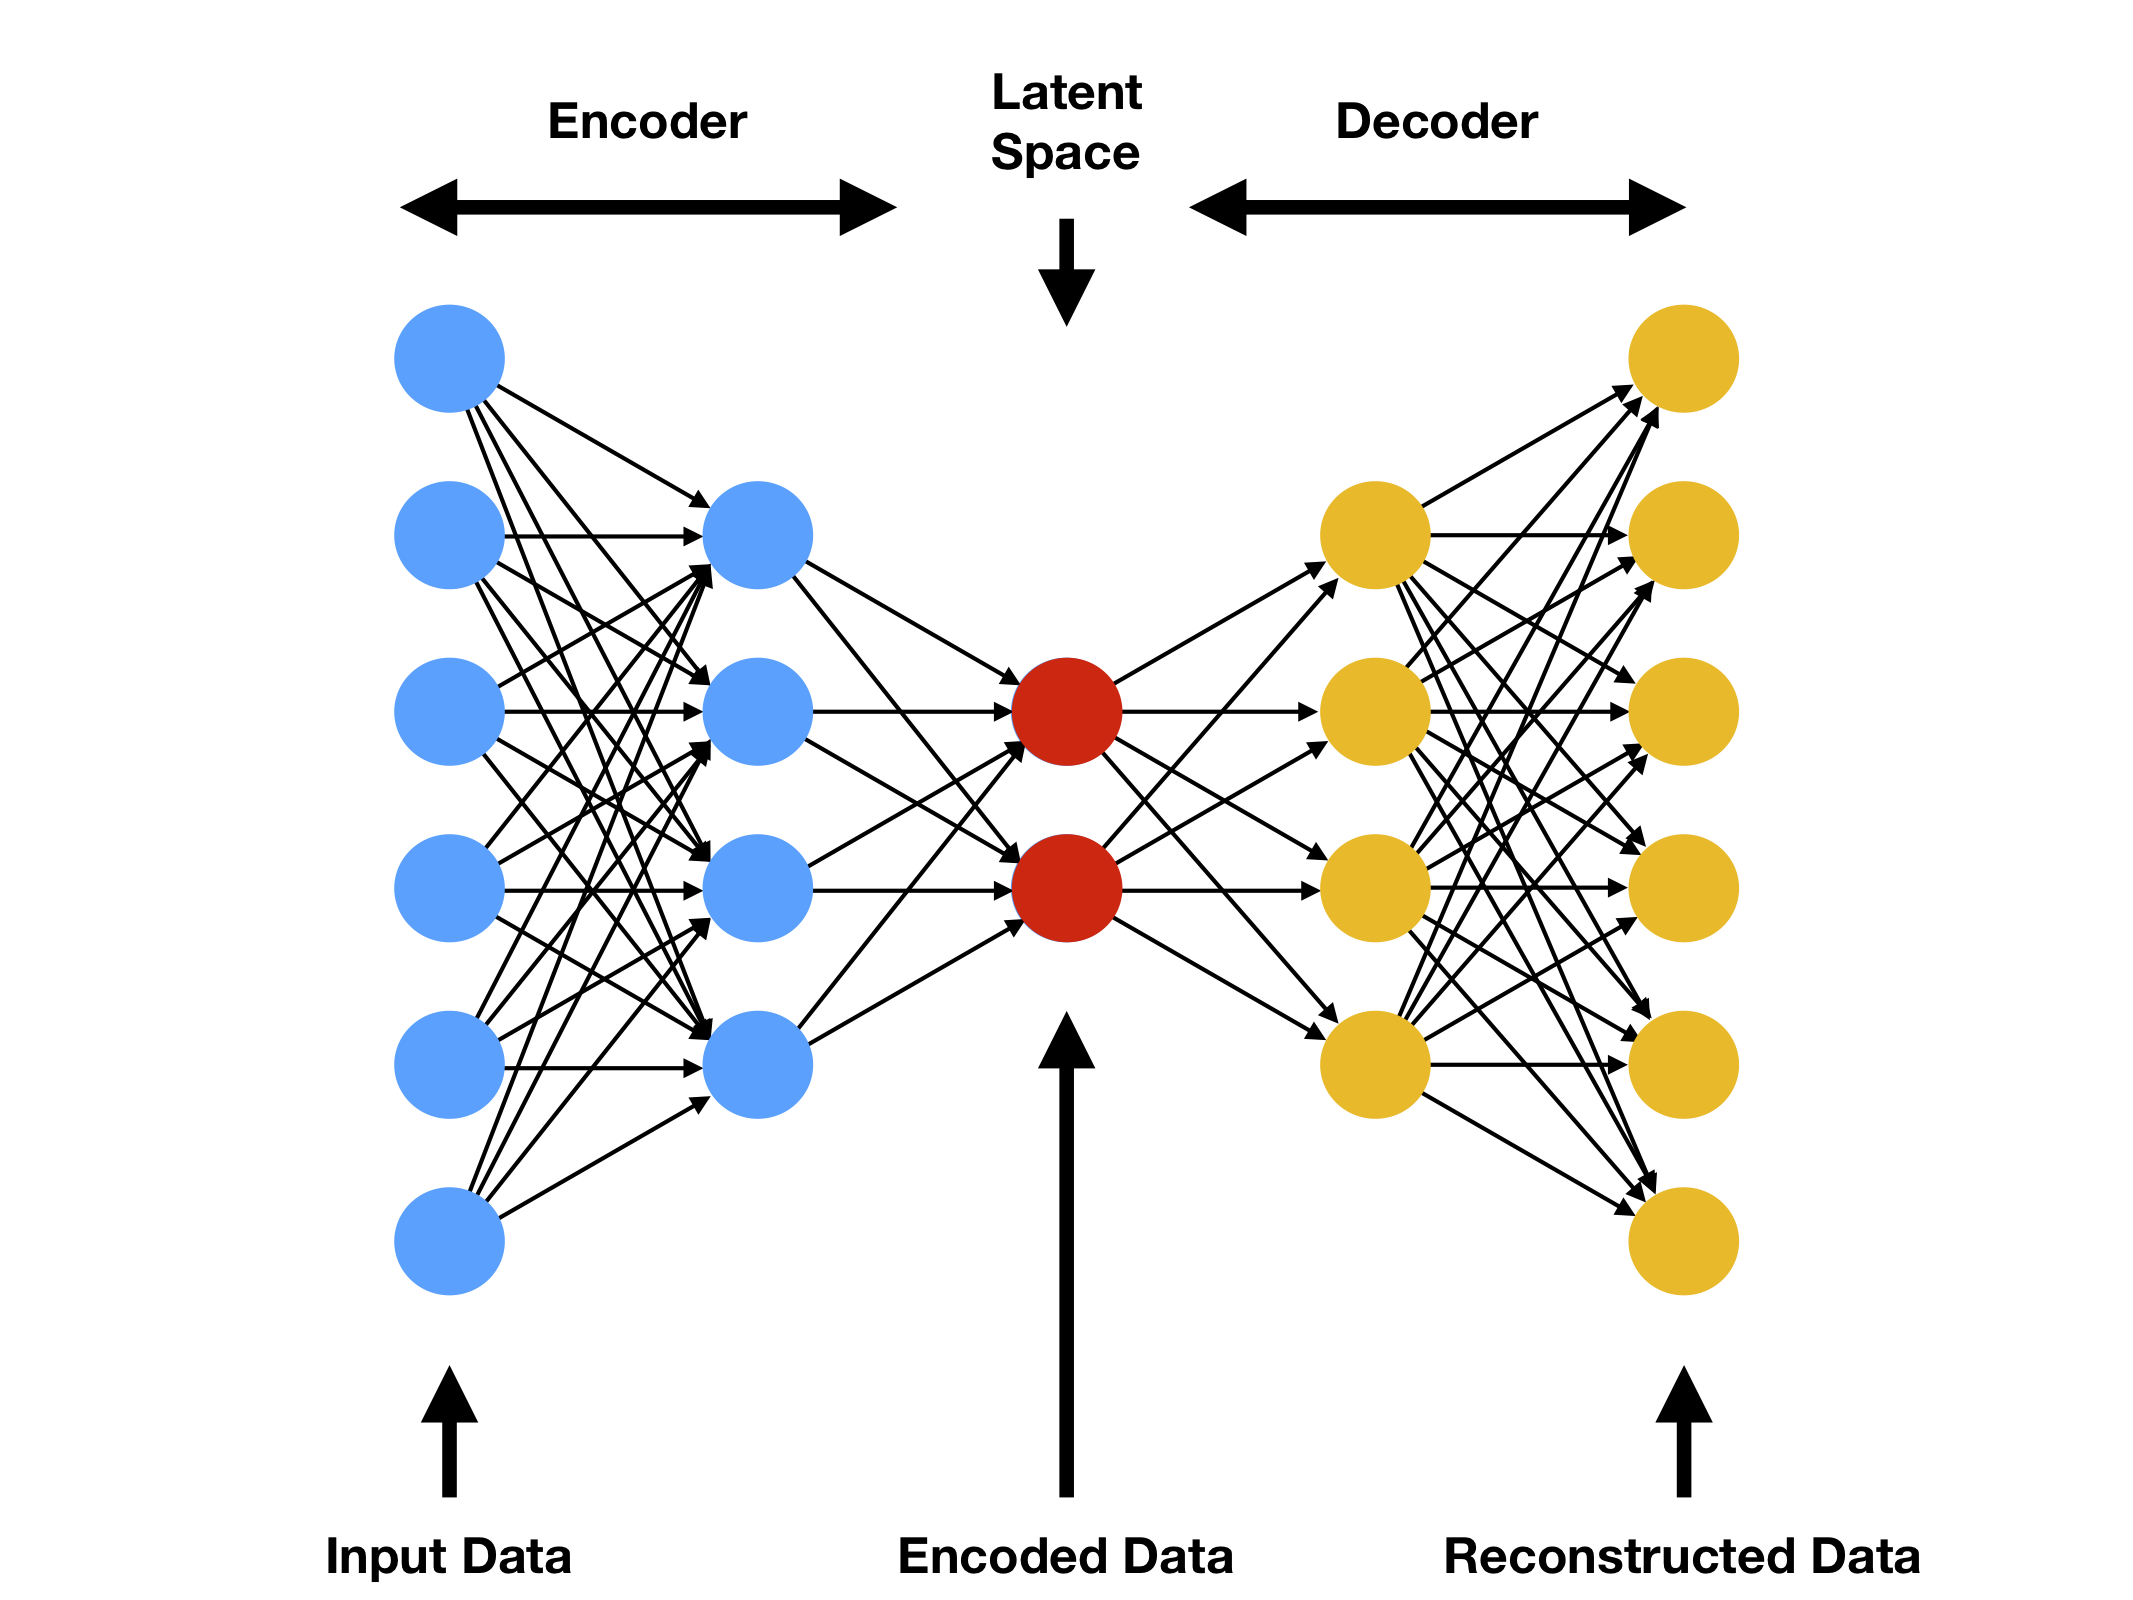
\includegraphics[width=0.8\textwidth]{doc_hw04/images/autoencoder.png}
    \caption{Arquitectura de un modelo de autoencoder}
    \label{fig:autoencoder}
\end{figure}

\subsection{\textit{Clustering}}

Ya a partir de las representaciones en un espacio de dimensiones reducido se procede a hacer la agrupación de los documentos para obtener grupos de tópicos relevantes. En este caso se realizaron pruebas con los algoritmos de \textit{Spectral Clustering}, \textit{Agglomerative Custering} y \textit{K-Means}. Sin embargo, a partir de los resultados presentados en \cite{DeepRepresentationClusteringTweets} y la posibilidad de recuperar los documentos más cercanos al centro del \textit{cluster} se decidió utilizar únicamente el algoritmo de \textit{K-Means}. De forma general, este algoritmo genera un número K de centroides aleatorios que agrupan los puntos (en este caso las representaciones de los documentos) más cercanos y los asocia a un \textit{cluster}. Posteriormente, y de forma iterativa, estos centroides se recalculan como la media de los puntos (o documentos) que agrupa el \textit{cluster} y vuelve a definir los \textit{clusters}. Vale la pena aclarar que un parámetro importante a ajustar en este algoritmo es el \textit{K} o el número de \textit{clusters}. Para esto se realizaron pruebas con distinto número de K y se evidencio la descripción (o \textit{keywords}) asociada a cada tópico para tomar esta decisión.

\subsection{\textit{Keywords Extraction}}

Finalmente, para poder describir el tópico (la agrupación o \textit{cluster} de documentos), se procedió a extraer las palabras que lo describen. Estos dan una idea de donde están concentrados los documentos más representativos del \textit{cluster}. De esta manera, se recuperó un número \textit{N} de documentos "relevantes", que son aquellos que se encuentran más cerca al centro del \textit{cluster}. Y, posteriormente, se extrajeron de esos documentos aquellos términos (o tokens) con mayor frecuencia dentro de esos documentos. Por último estos tópicos se presentan en el formato de \textit{wordcloud} para poder hacer más fácil su análisis.


\section{Resultados}
A continuación, se describen los resultados obtenidos del proceso de detección de temas tendencia con base en el procedimiento previamente descrito para cada uno de los idiomas seleccionados.

\subsection{Inglés}


\subsection{Español}

El proceso de \textit{clustering} hecho con base en el método K-means para el idioma español arrojó los resultados que se pueden ver en la figura \ref{fig:es_kmeans}. Se decidió probar diferente número de grupos con el fin de analizar el comportamiento y la exactitud con la que el algoritmos K-means es capaz de separarlos. Inicialmente, se probó con un total de cinco (\textit{véase fig} \ref{fig:es_kmeans_5}) \textit{clusters}, evidenciando que la separación entre los grupos color azul y morado era regular además del serio agravante de que a simple vista no es posible identificar el quinto \textit{cluster}. Se decidió entonces probar con un menor número grupos, o6bteniendo los resultados visibles en la figura \ref{fig:es_kmeans_4}, la cual resulta muy similar al caso previamente descrito.\\

Posteriormente, se redujo nuevamente el número de grupos definiéndolo en tres (\textit{véase fig} \ref{fig:es_kmeans_3}). En este caso las barreras de separación de cada grupo son completamente claras y son realmente pocos los documentos que las sobrepasan. Sin embargo, con base en el comportamiento a lo largo del tiempo se decidió intentar reducir el número de grupos a 2, obteniendo los resultados mostrados en la figura \ref{fig:es_kmeans_2}, en donde la división de \textit{clusters} es visible, pero la gráfica de comportamiento en el tiempo muestra mejores resultados.\\

\begin{figure}
     \centering
     \begin{subfigure}[b]{0.4\textwidth}
         \centering
         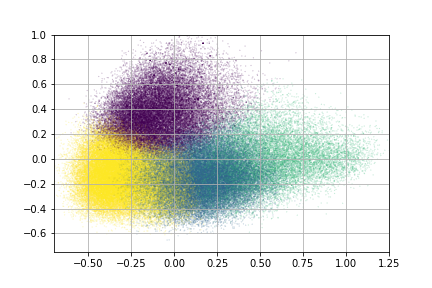
\includegraphics[width=\textwidth]{results/TopicDetection/es/PCA_2.png}
         \caption{2 clusters}
         \label{fig:es_kmeans_2}
     \end{subfigure}
     \hfill
     \begin{subfigure}[b]{0.4\textwidth}
         \centering
         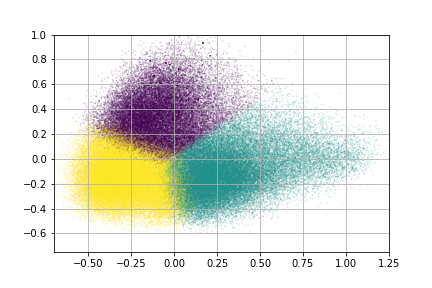
\includegraphics[width=\textwidth]{results/TopicDetection/es/PCA_3.png}
         \caption{3 clusters}
         \label{fig:es_kmeans_3}
     \end{subfigure}
     \hfill
     \begin{subfigure}[b]{0.4\textwidth}
         \centering
         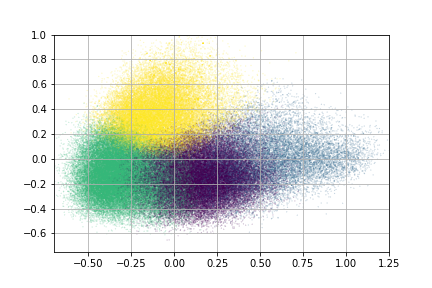
\includegraphics[width=\textwidth]{results/TopicDetection/es/PCA_4.png}
         \caption{4 clusters}
         \label{fig:es_kmeans_4}
     \end{subfigure}
     \hfill
     \begin{subfigure}[b]{0.4\textwidth}
         \centering
         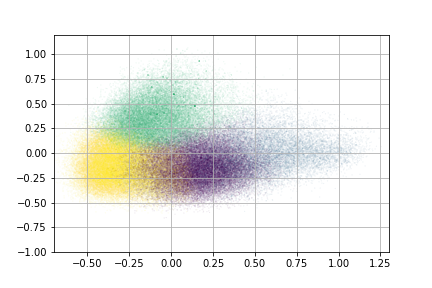
\includegraphics[width=\textwidth]{results/TopicDetection/es/PCA_5.png}
         \caption{5 clusters}
         \label{fig:es_kmeans_5}
     \end{subfigure}
        \caption{Resultados de K-means con diferente número de clusters}
        \label{fig:es_kmeans}
\end{figure}

Una vez seleccionado el número óptimo de grupos, se procede a extraer las palabras más representativas de cada uno de los grupos, mediante una nube de palabras. Se decide eliminar algunas que aparecen en mayoría en todos los \textit{clusters} con el fin de poder visualizar más aquellas que caracterizan cada uno.\\

\begin{figure}
    \centering
    \begin{subfigure}[b]{0.49\textwidth}
        \centering
        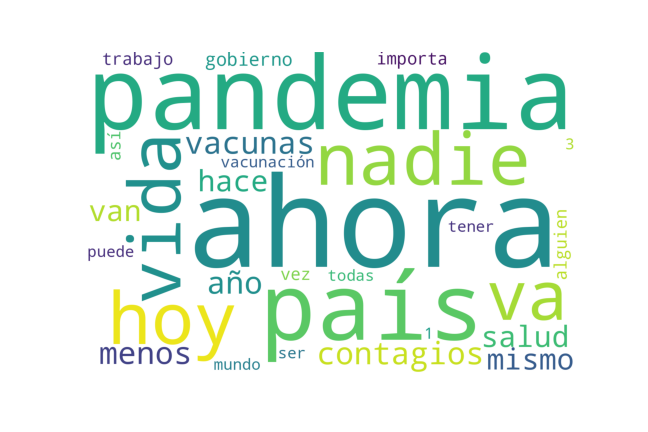
\includegraphics[width=\textwidth]{results/TopicDetection/es/cluster0.png}
        \caption{Cluster 0}
        \label{fig:es_c0}
    \end{subfigure}
    \hfill
    \begin{subfigure}[b]{0.49\textwidth}
        \centering
        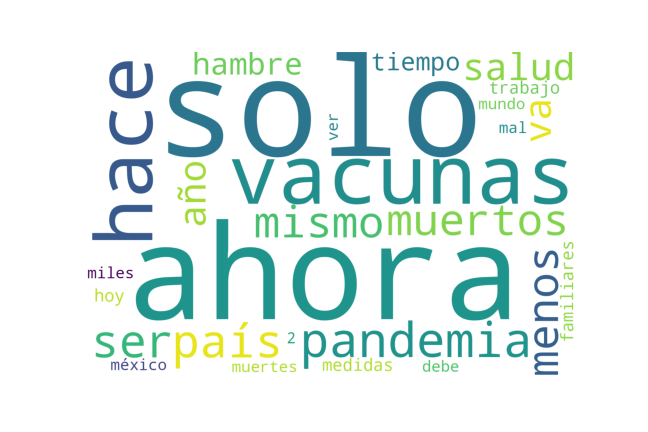
\includegraphics[width=\textwidth]{results/TopicDetection/es/cluster1.png}
        \caption{Cluster 1}
        \label{fig:es_c1}
    \end{subfigure}
    \hfill
    \begin{subfigure}[b]{0.49\textwidth}
        \centering
        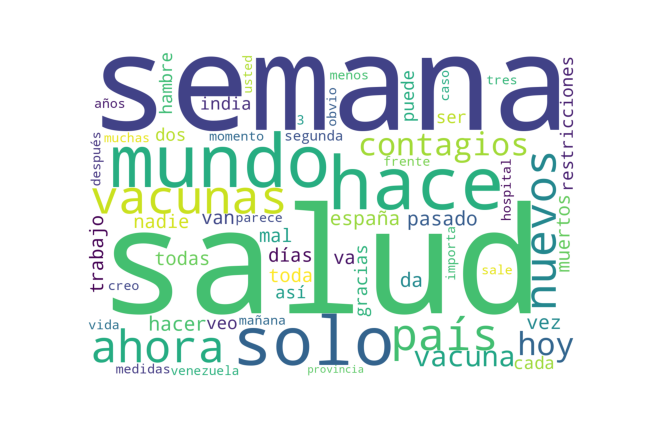
\includegraphics[width=\textwidth]{results/TopicDetection/es/cluster2.png}
        \caption{Cluster 2}
        \label{fig:es_c1}
    \end{subfigure}
    \hfill
    \begin{subfigure}[b]{0.49\textwidth}
        \centering
        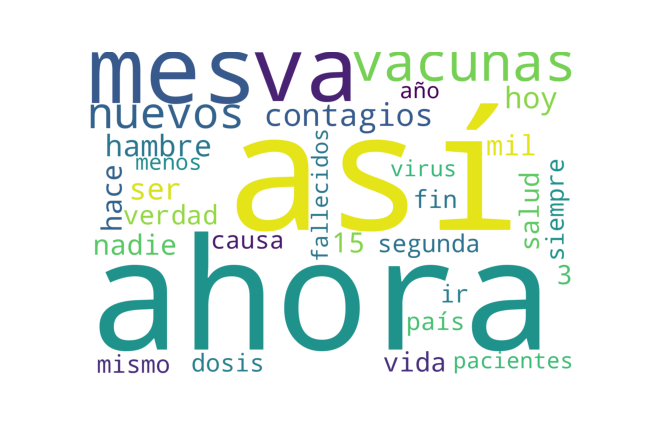
\includegraphics[width=\textwidth]{results/TopicDetection/es/cluster3.png}
        \caption{Cluster 3}
        \label{fig:es_c1}
    \end{subfigure}
    \caption{Principales palabras de cada uno de los clusters}
    \label{fig:es_clusters}
\end{figure}

Con base en las figuras \ref{fig:es_clusters} y \ref{fig:es_time} Es completamente evidente que el \textit{cluster} 1 crece fuertemente hacia el final de los meses evaluados, debido a la palabra vacunación, la cual ha sido tendencia últimamente y no aparece en el \textit{cluster} 0, cuya participación se reduce al final de los meses. De manera similar, los \textit{clusters} presentan una tendencia opuesta en el inicio de los meses, debido quizás a la palabra nuevos, que esta presente únicamente en el \textit{cluster} 1.

\begin{figure}
    \centering
    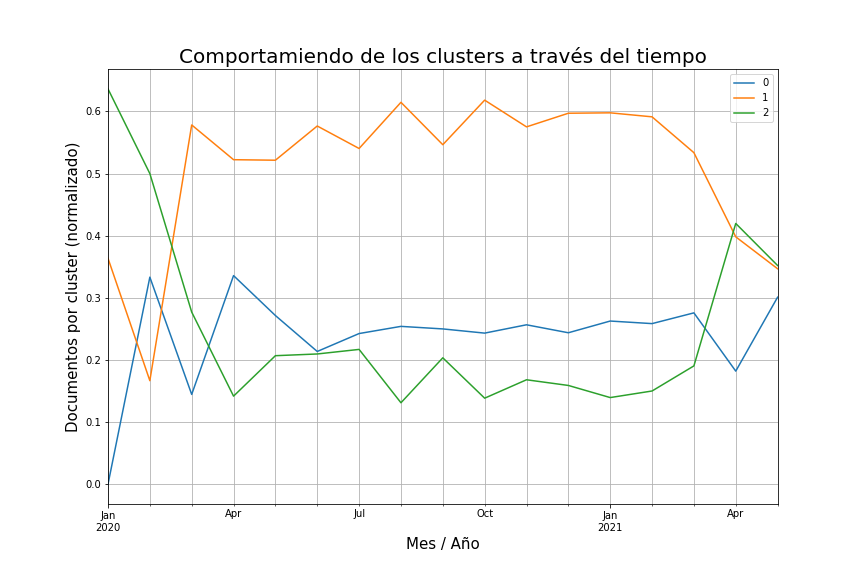
\includegraphics[width=0.9\textwidth]{results/TopicDetection/es/cluster_over_time.png}
    \caption{Comportamiento de los clusters en el tiempo}
    \label{fig:es_time}
\end{figure}

\subsection{Francés}

\section{Conclusiones}
Dentro del análisis de los datos que se obtuvieron al aplicar el modelo planteado con los diferentes conjuntos de datos fue posible obtener las siguientes conclusiones:
\begin{enumerate}
    \item Debido a la prominencia como \textit{lingua franca} a nivel mundial, los modelos desarrollados con este idioma obtuvieron resultados más evidentes y más cercanos a lo esperado que los de los idiomas Español y Francés. Esto se puede notar con las grandes diferencias entre las palabras claves de los \textit{clusters} para el idioma inglés. Por su parte, los otros dos idiomas las diferencias no fueron tan notorias, aunque si existieron puntos que demostraron la capacidad del modelo para extraer información.
    \item Al comparar el desempeño de los modelos de español y francés se notó cómo el primero fue capaz de realizar distinciones mucho mejor que el segundo. Una situación en la cuál se puede evidenciar este fenómeno es que el modelo en español contiene menos palabras repetidas entre los \textit{clusters}. Otro aspecto a tener en cuenta es la capacidad del modelo de identificar más clusters: mientras que se identificaron cuatro en español, sólo se identificaron tres en francés.
    \item Vale la pena tener en cuenta que puede haber un sesgo hacia ciertos términos debido a la época en la cual se recolectaron los datos. Dado que estos fueron recolectados en las últimas semanas hay un sesgo a tener más términos de este periodo de tiempo a datos de periodos anteriores. Si bien se buscó mitigar este fenómeno con la normalización de los datos, es posible que aún exista un sesgo hacia estos.
\end{enumerate}


\newpage
\bibliographystyle{unsrt}
\bibliography{biblist.bib}

\end{document}